\documentclass[../DS03.tex]{subfiles}%
\graphicspath{{./figures/}}%

\begin{document}%
\section[38]"E"{Réaction du dibromure de cuivre}

\enonce{%
On considère la dismutation du dibromure de cuivre selon l'équation~:
\[
	\ce{2CuBr_2_{\sol} = 2 CuBr_{\sol} + Br_2_{\gaz}}
\]
Cet équilibre se déroule dans un réacteur de volume constant $V = \SI{1.0}{L}$.
On mesure la pression à l'équilibre dans le réacteur, $P\ind{eq}$, en fonction
de la température $T$. Dans les cas d'un excès de \ce{CuBr2}, les résultats sont
compilés dans le tableau suivant~:
\begin{table}[htbp!]
	\centering
	% \renewcommand{\arraystretch}{2}
	% \aboverulesep = 0pt
	% \belowrulesep = 0pt
	\caption{Pression d'équilibre de la dismutation du dibromure de cuivre}
	\begin{tabular}{lcccc}
		\toprule
		$T~~(\si{K})$            &
		\num{473}                &
		\num{488}                &
		\num{503}                &
		\num{523}
		\\
		$P\ind{eq}~~(\si{mbar})$ &
		\num{52.6}               &
		\num{54.2}               &
		\num{140.8}              &
		\num{321.1}
		\\
		\bottomrule
	\end{tabular}
	\label{tab:data}
\end{table}
}%

\QR[4]{%
	Exprimer puis calculer la valeur de la constante d'équilibre à la température
	$T = \SI{200}{\degreeCelsius}$.
}{%
	Il est indiqué que les mesures sont effectuées avec un excès de \ce{CuBr2},
	qui est donc encore présent à la fin de la réaction. Il s'agit donc d'un état
	d'équilibre, et on donc appliquer la loi d'action des masses~:
	\begin{align*}
		K^\circ         & \stm{=} Q_{r,\eql}
		\\\Lra
		K^\circ         & \stm{=} \frac{a_{\ce{BR_2},\eql}\cdot a_{\ce{CuBr},\eql}^2}{a_{\ce{CuBr_2},\eql}}
		\\\Lra
		\Aboxed{K^\circ & \stm{=} \frac{p_{\ce{Br_2},\eql}}{p^\circ}}
		\makebox[0pt][l]{$\qav
				\left\{
				\begin{array}{rcl}
					p_{\ce{Br_2},\eql} & = & \SI{52.6e-3}{bar}
					\\
					p^\circ            & = & \SI{1}{bar}
				\end{array}
				\right.$}
		\\
		\AN
		\makebox[0pt][l]{$\xul{\phantom{K^\circ = \num{52.6e-3}}}$}
		K^\circ         & \stm{=} \num{52.6e-3}
	\end{align*}
}%

\enonce{%
	On introduit une quantité de matière $n_1 = \SI{2.00e-3}{mol}$ de \ce{CuBr2}
	dans le réacteur. La température est supposée constante à \SI{200}{\degreeCelsius}.
}%
\QR[13]{%
	Déterminer la composition et la pression à l'état final. Comment s'appelle cet
	état final~?
}{%
	On suppose un état d'équilibre. La pression finale vaut alors
	\SI{52.6}{mbar} d'après le tableau de valeurs. On peut en déduire la
	quantité de dibrome formé, et donc l'avancement grâce à un tableau~:
	\begin{center}
		\def\rhgt{0.50}
		\centering
		\begin{tabularx}{.7\linewidth}{|l|c||YdYdY|}
			\hline
			\multicolumn{2}{|c||}{
				$\xmathstrut{\rhgt}$
			\textbf{Équation} \pt{1}+\pt{1}} &
			$2\ce{CuBr_2_{\sol}}$            & $=$                    &
			$2\ce{CuBr_{\sol}}$              & $+$                    &
			$\ce{Br_2_{\gaz}}$                                          \\
			\hline
			$\xmathstrut{\rhgt}$
			Initial                          & $\xi = 0$              &
			$n_1$                            & \vline                 &
			$0$                              & \vline                 &
			$0$
			\tikzmark{MA}
			\\
			\hline
			$\xmathstrut{\rhgt}$
			Final                            & $\xi_f$                &
			$n_1 - 2\xi_{f}$                 & \vline                 &
			$2\xi_{f}$                       & \vline                 &
			$\xi_{f}$
			\tikzmark{MB}
			\\
			\hline
			$\xmathstrut{\rhgt}$
			Final (\si{mmol})                & $\xi_f = \xi\ind{max}$ &
			$0$                              & \vline                 &
			$\num{2.00}$                     & \vline                 &
			$\num{1.00}$
			\tikzmark{MC}
			\\
			\hline
		\end{tabularx}
	\end{center}
	\tikz[remember picture, overlay]
	\node[above right=-8pt and 35pt of pic cs:MA] {\pt{1}}
	;
	\tikz[remember picture, overlay]
	\node[above right=-8pt and 35pt of pic cs:MB] {\pt{1}}
	;
	\tikz[remember picture, overlay]
	\node[above right=-8pt and 35pt of pic cs:MC] {\pt{1}}
	;
	\begin{gather*}
		\beforetext{Ainsi, on trouve}
		n_{\ce{Br_2},eq} = \boxed{\xi\ind{eq} \stm{=} \frac{P\ind{eq}V}{RT}}
		\qav
		\left\{
		\begin{array}{rcl}
			P\ind{eq} & = & \SI{52.6e2}{Pa}
			\\
			V         & = & \SI{1.0e-3}{m^3}
			\\
			R         & = & \SI{8.314}{J.K^{-1}.mol^{-1}}
			\\
			T         & = & \SI{473}{K}
		\end{array}
		\right.\\
		\AN
		\xul{
			\xi\ind{eq} \stm{=} \SI{1.34}{mmol}
		}
	\end{gather*}
	Or, on trouve facilement l'avancement maximal~:
	\begin{gather*}
		n_1 - 2\xi\ind{max} = 0
		\Lra
		\boxed{\xi\ind{max} \stm{=} \frac{n_1}{2}}
		\Ra
		\xul{\xi\ind{max} \stm{=} \SI{1.00}{mmol}} < \xi\ind{eq}
		\\\beforetext{Ainsi,}
		\boxed{\xi_f \stm{=} \xi\ind{max}}
		\qquad \text{\textbf{rupture d'équilibre}} \quad \pt{1}
	\end{gather*}
	On complète alors la dernière ligne du tableau. Quant à la pression, on la
	calcule avec la quantité de dibrome à l'état final, $n_{\ce{Br_2},f} =
		\SI{1.00}{mmol}$~:
	\[
		\boxed{P_f \stm{=} \frac{n_{\ce{Br_2},f}RT}{V}}
		\Ra
		\xul{P_f \stm{=} \SI{3.9e-2}{bar}}
	\]
}%

\begin{blocQR}
	\item \enonce{%
		Préciser l'évolution du système précédent pour les trois modifications
		suivantes~:
	}%
	\QR[2]{%
		Ajout de \ce{CuBr2} à $T$ et $P$ constantes.
	}{%
		Le système était en rupture d'équilibre. L'ajout de réactif va donc
		entraîner l'évolution en sens direct \pt{1}, et selon la quantité ajoutée le
		système peut aboutir à une nouvelle rupture d'équilibre ou à un état
		d'équilibre. \pt{1}
	}%
	\QR[1]{%
		Ajout de \ce{CuBr} à $T$ et $P$ constantes.
	}{%
		Le système est en rupture d'équilibre car le réactif est limitant. Ajouter
		un produit ne change rien. \pt{1}
	}%
	\QR[1]{%
		Ajout de \ce{Br2} à $T$ et $P$ constantes.
	}{%
		Le système est en rupture d'équilibre car le réactif est limitant. Ajouter
		un produit ne change rien. \pt{1}
	}%
\end{blocQR}

\enonce{%
	On considère maintenant une quantité de matière initiale de \ce{CuBr2} $n_2 =
		\SI{1.00e-2}{mol}$ dans les mêmes conditions.
}%

\QR[6]{%
	Déterminer la composition et la pression à l'état final. Comment s'appelle cet
	état final~?
}{%
	De la même manière que précédemment, on a $\xi\ind{eq}$ inchangé \pt{1},
	seulement on trouve $\xi\ind{max} \stm[-1]{=} \SI{5.00}{mmol} > \xi\ind{eq}$~;
	ainsi $\xi_f = \xi\ind{eq}$ \pt{1}, on atteint donc un \textbf{état
		d'équilibre} \pt{1} et on peut compléter le tableau d'avancement~:
	\begin{center}
		\def\rhgt{0.50}
		\centering
		\begin{tabularx}{.7\linewidth}{|l|c||YdYdY|}
			\hline
			\multicolumn{2}{|c||}{
				$\xmathstrut{\rhgt}$
			\textbf{Équation}}    &
			$2\ce{CuBr_2_{\sol}}$ & $=$                   &
			$2\ce{CuBr_{\sol}}$   & $+$                   &
			$\ce{Br_2_{\gaz}}$                                                                  \\
			\hline
			$\xmathstrut{\rhgt}$
			Initial               & $\xi = 0$             & $n_2$ & \vline & $0$ & \vline & $0$
			% \tikzmark{MA}
			\\
			\hline
			$\xmathstrut{\rhgt}$
			Final (\si{mmol})     & $\xi_f = \xi\ind{eq}$ &
			$\num{7.32}$          & \vline                &
			$\num{2.68}$          & \vline                &
			$\num{1.34}$
			\tikzmark{MD}
			\\
			\hline
		\end{tabularx}
	\end{center}
	% \tikz[remember picture, overlay]
	% \node[above right=-8pt and 35pt of pic cs:MA] {\pt{1}}
	% ;
	\tikz[remember picture, overlay]
	\node[above right=-8pt and 35pt of pic cs:MD] {\pt{1}}
	;
	\begin{gather*}
		\beforetext{On a alors}
		\boxed{P_f = P\ind{eq}}
		\Ra
		\xul{P_f \stm{=} \SI{52.6}{mbar}}
	\end{gather*}
}%

\begin{blocQR}
	\item \enonce{%
		Préciser l'évolution du système précédent pour les trois modifications
		suivantes~:
	}%
	\QR[1]{%
		Ajout de \ce{CuBr2} à $T$ et $P$ constantes.
	}{%
		Le système est à l'équilibre, et l'ajout d'un constituant solide ne modifie
		pas le quotient de réaction. Il n'y a donc pas d'évolution. \pt{1}
	}%
	\QR[1]{%
		Ajout de \ce{CuBr} à $T$ et $P$ constantes.
	}{%
		Le système est à l'équilibre, et l'ajout d'un constituant solide ne modifie
		pas le quotient de réaction. Il n'y a donc pas d'évolution. \pt{1}
	}%
	\QR[2]{%
		Ajout de \ce{Br2} à $T$ et $P$ constantes.
	}{%
		Le système est à l'équilibre, et l'ajout d'un constituant gazeux augmente le
		quotient de réaction \pt{1}. Celui-ci devient donc plus grand que la constante
		d'équilibre, et il y a alors \textbf{évolution en sens indirect}. \pt{1}
	}%
\end{blocQR}

\QR[7]{%
	On souhaite maintenant déterminer l'influence du volume du réacteur sur la
	pression mesurée à l'état final $P_f$, à température constante et à partir
	d'un état initial contenant $n_0$ moles de \ce{CuBr2}.
	\smallbreak
	Tracer le graphique $P_f = f(V)$ et préciser les coordonnées du point
	remarquable.
}{%
	\noindent
	\begin{minipage}[c]{.48\linewidth}
		Pour un excès de \ce{CuBr2}, l'état final sera un état d'équilibre donc la
		pression sera constante, avec
		\[
			P_f = K^\circ P^\circ
			\qquad \pt{1}
		\]
		En revanche, si \ce{CuBr2} est en défaut, il y a rupture d'équilibre, et on
		aura
		\[
			n_{\ce{Br_2},f} = \xi\ind{max} \stm{=} \frac{n_0}{2}
			\Ra
			P_f \stm{=} \frac{n_0RT}{2V}
		\]
		La limite de défaut/excès de \ce{CuBr2} est trouvée lorsque la quantité
		introduite permet tout juste d'atteindre l'état d'équilibre tout en ayant donc
		la pression maximale~; soit $V\ind{lim}$ le volume limite, on a alors
		\[
			\frac{n_0RT}{2V\ind{lim}} \stm{=} K^\circ P^\circ
			\Lra
			\boxed{V\ind{lim} \stm{=} \frac{n_0RT}{2K^\circ P^\circ}}
		\]
		D'où le graphique~:
	\end{minipage}
	\hfill
	\begin{minipage}[c]{.48\linewidth}
		\begin{center}
			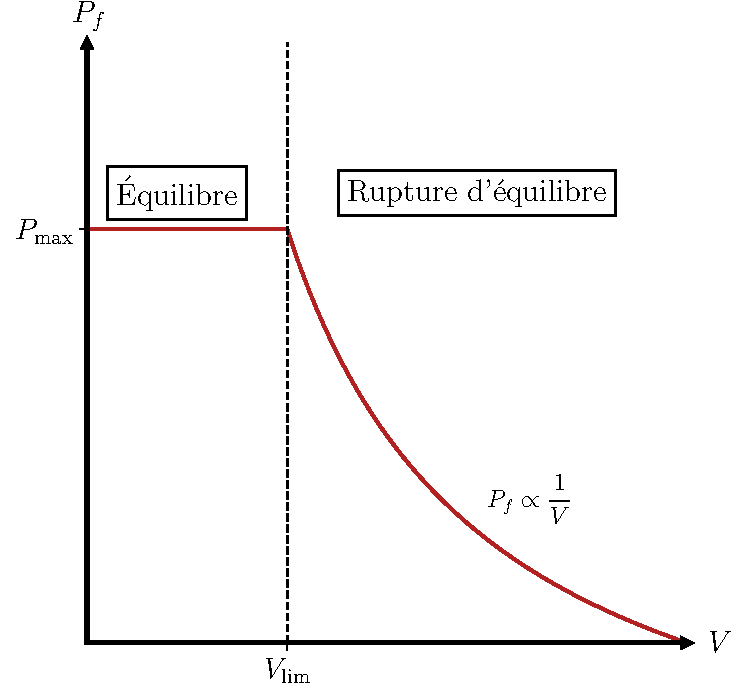
\includegraphics[width=\linewidth]{pf_V}
			\captionof{figure}{Tracé $P_f = f(V)$. \protect\pt{1} + \protect\pt{1}}
			\label{fig:pf_V}
		\end{center}
	\end{minipage}
}%

\end{document}%
